\section{Regularización}

\subsection{Diagnóstico con curvas de entrenamiento y validación}

La Figura~\ref{fig:curvas-av4} compara exactitud y entropía cruzada para cada
modelo. Se muestran todas las épocas ejecutadas y se marca la época seleccionada
por F1 macro. No se confunde la última época con el checkpoint final evaluado.
En una fase de sobreajuste, el modelo sigue reduciendo su error de entrenamiento
sin obtener la misma mejora en validación; en particular, una pérdida de validación
que aumenta revela errores más confiados aunque la exactitud cambie poco.

\begin{itemize}
\item \textbf{MLP de referencia}: la menor pérdida de validación fue 3.339 en la época 76. Al terminar, la pérdida de entrenamiento fue 3.595 y la de validación 3.345; la exactitud de entrenamiento fue 11.78\% y la de validación 15.41\%. Estas curvas deben interpretarse junto con F1 macro; no se concluye sobreajuste solo por una diferencia entre exactitudes.
\item \textbf{CNN original}: la menor pérdida de validación fue 1.520 en la época 53. Al terminar, la pérdida de entrenamiento fue 0.937 y la de validación 1.609; la exactitud de entrenamiento fue 71.17\% y la de validación 62.53\%. La reducción de la pérdida de entrenamiento junto con una pérdida de validación mayor que su mínimo es evidencia de sobreajuste en la fase final.
\item \textbf{CNN + 2 convoluciones}: la menor pérdida de validación fue 1.658 en la época 31. Al terminar, la pérdida de entrenamiento fue 0.564 y la de validación 2.024; la exactitud de entrenamiento fue 82.66\% y la de validación 60.48\%. La reducción de la pérdida de entrenamiento junto con una pérdida de validación mayor que su mínimo es evidencia de sobreajuste en la fase final.
\item \textbf{CNN + AdamW + LR}: la menor pérdida de validación fue 1.494 en la época 52. Al terminar, la pérdida de entrenamiento fue 0.785 y la de validación 1.512; la exactitud de entrenamiento fue 76.16\% y la de validación 64.41\%. Estas curvas deben interpretarse junto con F1 macro; no se concluye sobreajuste solo por una diferencia entre exactitudes.
\end{itemize}

\begin{figure*}[p]
\centering
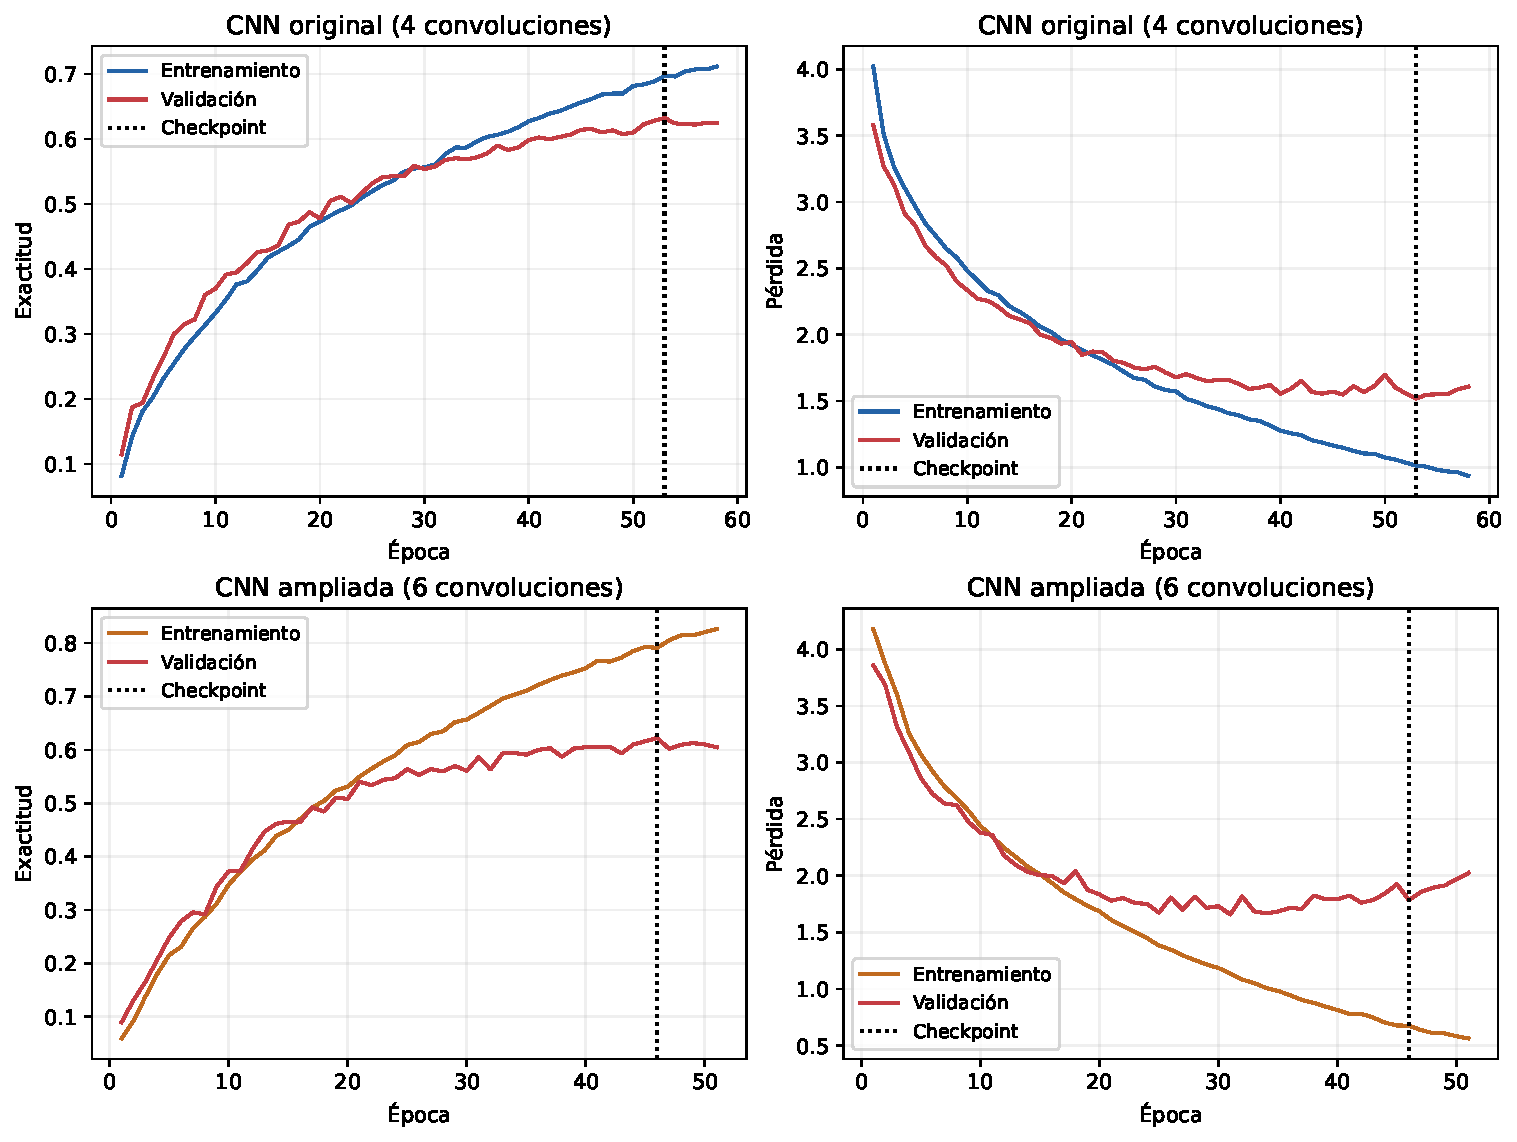
\includegraphics[width=\textwidth,keepaspectratio]{avance4_2026-10-21/figures/comparacion_original_ampliada.pdf}
\caption{CNN original y CNN ampliada: curvas reales por época. El entrenamiento usa aumentos y dropout; la
validación no. Las líneas verticales marcan el mejor checkpoint por F1 macro.}
\label{fig:curvas-av4}
\end{figure*}

\begin{figure*}[p]
\centering
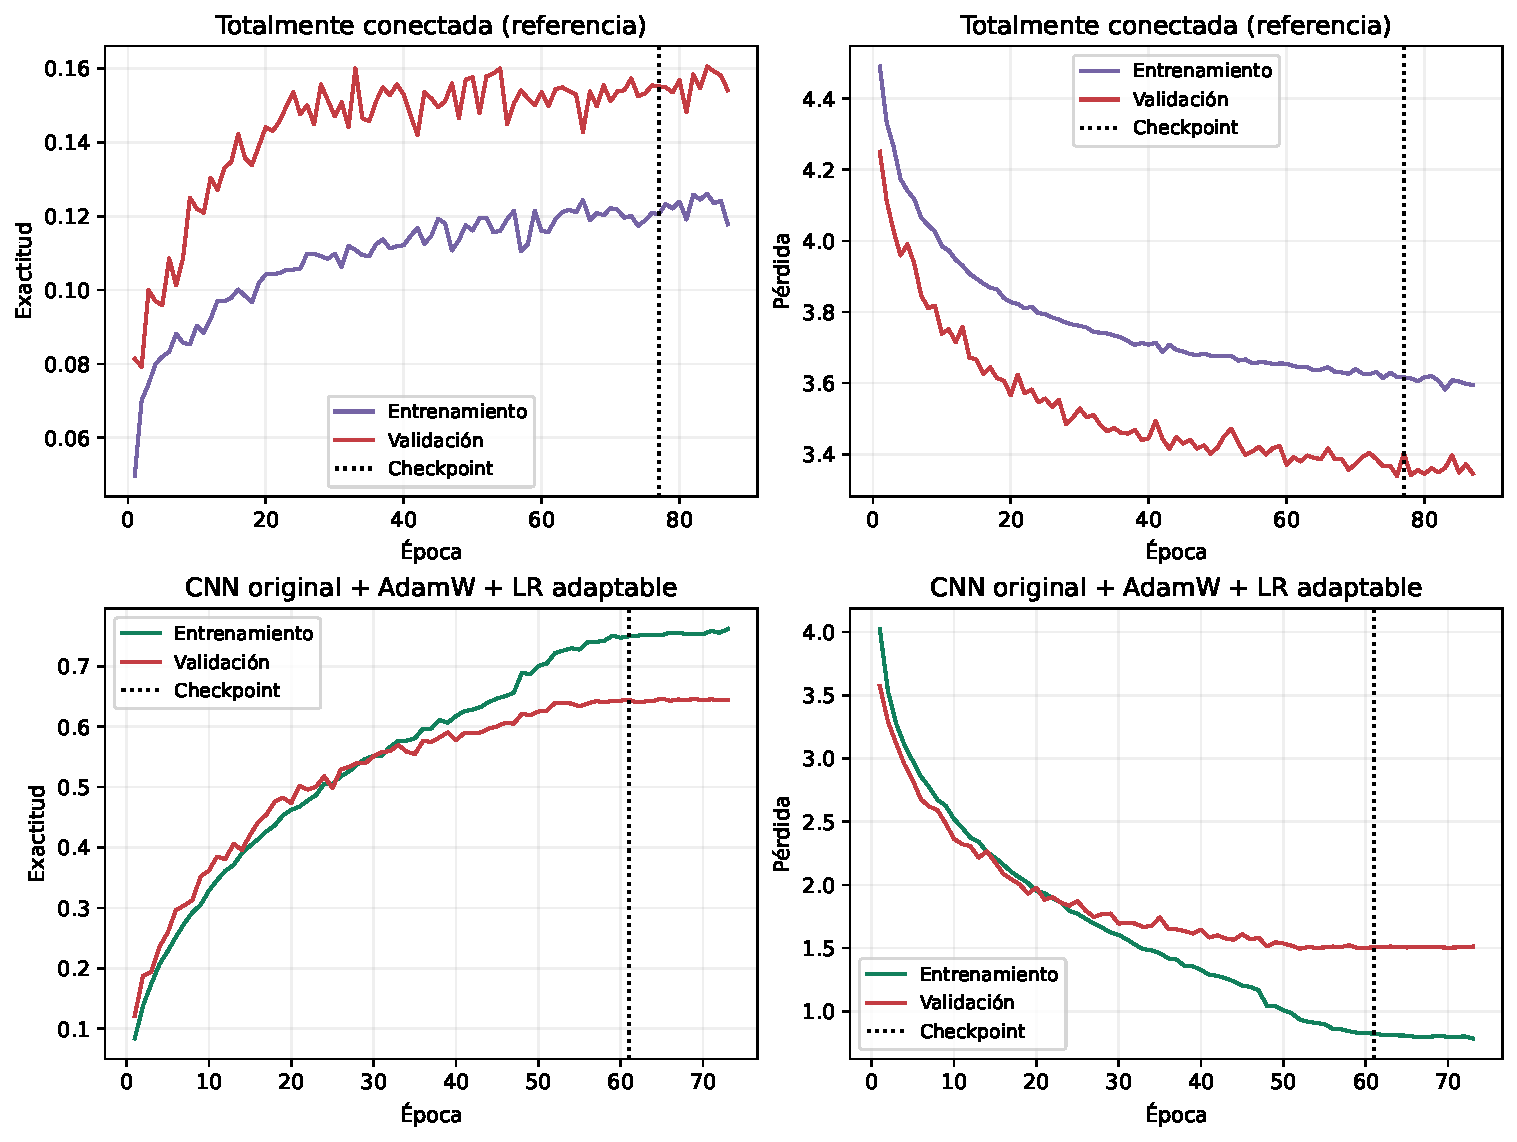
\includegraphics[width=\textwidth,keepaspectratio]{avance4_2026-10-21/figures/comparacion_referencia_regularizada.pdf}
\caption{Curvas de la referencia totalmente conectada y la CNN con la intervención
combinada de regularización. Se mantienen separados sus checkpoints y métricas.}
\label{fig:curvas-ref-reg-av4}
\end{figure*}

\subsection{Técnicas aplicadas y efecto medido}

Todos los modelos usan dropout de 0.5 antes de la salida, aumentos de datos
solo en entrenamiento y parada temprana con restauración del mejor checkpoint.
No se entrenó una ablación sin dropout ni sin aumentos; por eso no se atribuye
por separado una mejora numérica a estas dos técnicas.

La intervención adicional conserva la CNN de cuatro convoluciones, pero utiliza
AdamW con decaimiento de pesos de 0.01 sobre matrices de pesos, excluyendo sesgos.
Se trata de decaimiento desacoplado y no de añadir un término L2 a la pérdida
mostrada. Además, reduce la tasa de aprendizaje a la mitad cuando la pérdida de
validación no mejora durante dos evaluaciones, hasta un mínimo de $10^{-5}$.
La paciencia de parada temprana pasa de 5 a 12 evaluaciones para permitir actuar
a esa reducción. Esta es una intervención combinada: no permite aislar cuánto
aportó el decaimiento, el ajuste de tasa o la paciencia.

Frente a la CNN original, la variante regularizada cambia la exactitud de 63.25\% a 64.44\% (+1.19 puntos porcentuales) y F1 macro de 0.5740 a 0.5745 (+0.0005). Ambos valores se obtienen de los respectivos checkpoints seleccionados por F1 macro sobre la misma validación.

La diferencia de F1 macro es pequeña. Con una sola semilla no se considera evidencia de una mejora robusta o estadísticamente significativa.

Una mejora de exactitud acompañada de una caída de F1 macro no se interpreta como mejora general: el criterio prioritario es el desempeño equilibrado entre las 104 clases. Tampoco se afirma que el sobreajuste desaparezca; se compara la evidencia de las curvas y se conserva el checkpoint que generaliza mejor según la validación disponible.

\begin{figure*}[htbp]
\centering
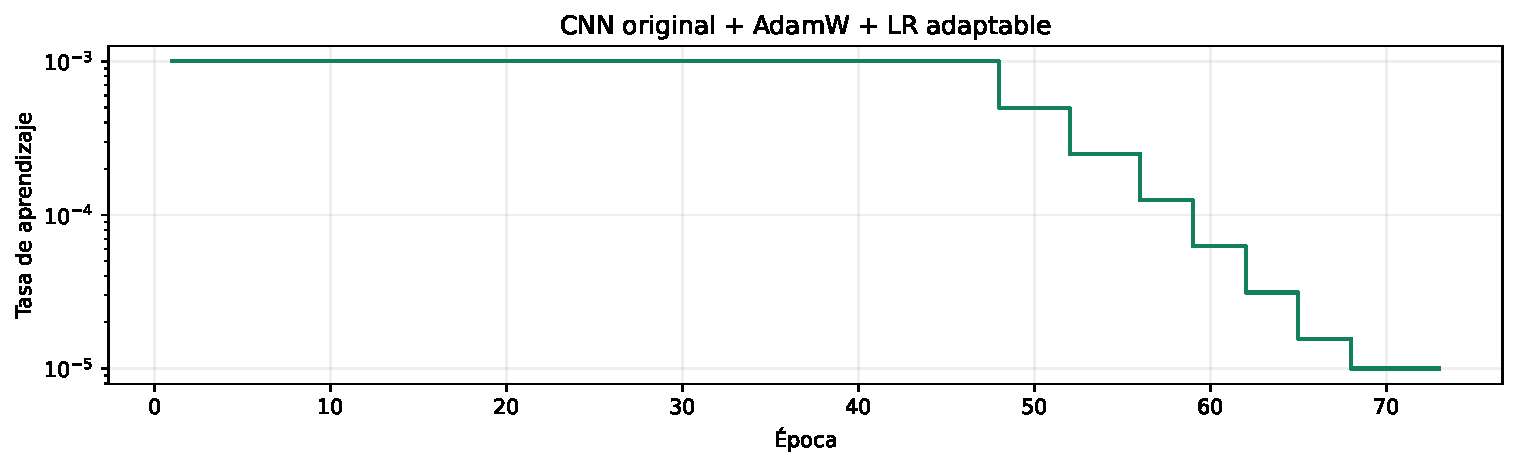
\includegraphics[width=\textwidth]{avance4_2026-10-21/figures/cnn_regularizada/tasa_aprendizaje.pdf}
\caption{Tasa de aprendizaje realmente utilizada en cada época de la variante regularizada. Las reducciones responden al estancamiento de la pérdida de validación.}
\label{fig:lr-av4}
\end{figure*}
